\documentclass[12pt,a4paper]{article}
% ==========================================
% PACKAGES ET CONFIGURATION DE BASE
% ==========================================
\usepackage[utf8]{inputenc}
\usepackage[T1]{fontenc}
\usepackage[french]{babel}
\usepackage{geometry}
\geometry{top=2.5cm, bottom=2.5cm, left=2.5cm, right=2.5cm}
\usepackage{graphicx}
\usepackage{xcolor}
\usepackage{hyperref}
\usepackage{titlesec}
\usepackage{listings}
\usepackage{tcolorbox}
\tcbuselibrary{skins,breakable}
\usepackage{fancyhdr}
\usepackage{booktabs}
\usepackage{amsmath,amssymb}
\usepackage{float}
\usepackage{tikz}
\usetikzlibrary{positioning,arrows.meta,shapes.geometric,fit,backgrounds}

% ==========================================
% CONFIGURATION DES STYLES & HYPERREF
% ==========================================
\hypersetup{
    colorlinks=true,
    linkcolor=black,
    filecolor=magenta,      
    urlcolor=blue,
    pdftitle={Rapport de Tests de Mutation — EduStream},
}

% Personnalisation des titres
\titleformat{\section}{\color{blue!70!black}\normalfont\Large\bfseries}{\thesection}{1em}{}
\titleformat{\subsection}{\color{blue!50!black}\normalfont\large\bfseries}{\thesubsection}{1em}{}
\titleformat{\subsubsection}{\normalfont\normalsize\bfseries}{\thesubsubsection}{1em}{}

% Style pour les blocs de code TypeScript / React
\lstset{
    basicstyle=\ttfamily\small,
    breaklines=true,
    frame=single,
    backgroundcolor=\color{gray!5},
    rulecolor=\color{gray!30},
    keywordstyle=\color{blue!80!black}\bfseries,
    commentstyle=\color{green!60!black}\itshape,
    stringstyle=\color{orange!90!black}
}

% Langage TypeScript (absent de listings) et accents UTF-8 dans les blocs de code
\lstdefinelanguage{typescript}{
    keywords={import,from,export,class,const,let,var,function,async,await,return,if,else,throw,new,private,static,readonly,interface,type,describe,it,expect,beforeEach,afterEach,true,false,void,string,number,boolean},
    sensitive=true,
    comment=[l]{//},
    morecomment=[s]{/*}{*/},
    morestring=[b]',
    morestring=[b]"
}
\lstset{
    literate=
    {é}{{\'e}}1 {è}{{\`e}}1 {ê}{{\^e}}1 {à}{{\`a}}1 {â}{{\^a}}1 {ù}{{\`u}}1
    {û}{{\^u}}1 {ô}{{\^o}}1 {î}{{\^i}}1 {ç}{{\c c}}1 {É}{{\'E}}1 {À}{{\`A}}1
}

% Encadré personnalisé pour le fonctionnement des tests
\tcbset{
    preuvebox/.style={
        colback=blue!5!white,
        colframe=blue!70!black,
        fonttitle=\bfseries,
        title=Détails du Fonctionnement et Validation du Test :,
        arc=4mm,
        boxrule=1pt,
        left=4pt,
        right=4pt,
        top=4pt,
        bottom=4pt
    },
    terminalbox/.style={
        colback=black!90!white,
        colframe=black!95!white,
        coltext=green!80!white,
        fonttitle=\bfseries\ttfamily,
        title=Terminal - Exécution Vitest v5.0.1,
        arc=2mm,
        boxrule=1pt
    }
}

% Figure : insérée uniquement si le fichier image existe
\newcommand{\capturefig}[3]{%
  \IfFileExists{#1}{%
  \begin{figure}[H]
  \centering
  \includegraphics[width=13.5cm,height=17cm,keepaspectratio]{#1}
  \caption{#2}
  \label{#3}
  \end{figure}}{}}
\tcbset{
    echecbox/.style={
        colback=black!90!white, colframe=red!60!black, coltext=red!35!white,
        fonttitle=\bfseries\ttfamily, arc=2mm, boxrule=1pt, breakable
    }
}

% En-têtes et pieds de page
\pagestyle{fancy}
\fancyhf{}
\fancyhead[L]{\small École Mohammadia d'Ingénieurs --- Génie Informatique}
\fancyhead[R]{\small Tests de Mutation --- EduStream}
\fancyfoot[C]{\thepage}
\renewcommand{\headrulewidth}{0.4pt}

\begin{document}

% ==========================================
% PAGE DE GARDE
% ==========================================
\begin{titlepage}

    \begin{flushleft}
        \IfFileExists{logo.jpg}{
\includegraphics[width=8cm]{logo.jpg}}{}
    \end{flushleft}

    \begin{center}
        \vspace*{0.5cm}

        \Large{\textbf{École Mohammadia d'Ingénieurs}}\\[0.5cm]
        \large{Département de Génie Informatique}\\[2.5cm]

        \rule{\textwidth}{1pt}\\[0.7cm]
        \huge{\textbf{Tests de Mutation}}\\[0.3cm]
        \Large{\textbf{Mesurer la qualité réelle des tests unitaires d'EduStream}}\\[0.4cm]
        \rule{\textwidth}{1pt}\\[2.5cm]

        \begin{minipage}{0.4\textwidth}
            \begin{flushleft} \large
                \textbf{Réalisé par :}\\
                BAKLOUL Mohamed\\
                HARBAL Salama
            \end{flushleft}
        \end{minipage}
        ~
        \begin{minipage}{0.4\textwidth}
            \begin{flushright} \large
                \textbf{Encadré par :}\\
                Pr. RETBI
            \end{flushright}
        \end{minipage}\\[2.5cm]

        \vfill

        \large{Année Universitaire : 2026 - 2027}\\[1cm]
    \end{center}
\end{titlepage}

\newpage
\tableofcontents
\newpage

% ==========================================
% 1. INTRODUCTION
% ==========================================
\section{Pourquoi des Tests de Mutation ?}
Le rapport précédent a montré que la suite Vitest passait avec une couverture de lignes de $75{,}81\,\%$. Cette couverture mesure seulement les lignes \textbf{exécutées} pendant les tests, pas les comportements réellement \textbf{vérifiés}. Un test qui appelle une fonction sans contrôler son résultat fait monter la couverture sans protéger le code.

Le test de mutation répond à la question : \textit{\og si le code contenait une erreur, mes tests la détecteraient-ils ? \fg{}} Le principe est le suivant :
\begin{enumerate}
    \item on introduit volontairement une petite erreur dans le code (un \textbf{mutant}), par exemple remplacer \texttt{<} par \texttt{<=}, supprimer une instruction ou vider un message d'erreur ;
    \item on relance les tests unitaires ;
    \item si au moins un test échoue, le mutant est \textbf{tué} (les tests ont détecté l'erreur) ; si tous les tests passent, le mutant \textbf{survit} : une partie du comportement n'est vérifiée par personne.
\end{enumerate}
\[
\text{score de mutation} = \frac{\text{mutants tués}}{\text{mutants tués} + \text{mutants survivants}}
\]

\subsection{Règle métier retenue}
EduStream est un projet de test : \textbf{une carte qui passe la validation (algorithme de Luhn, date d'expiration, CVV, titulaire) est acceptée}. Aucun paiement valide ne doit être refusé par la simulation de paiement (ni au hasard, ni parce que la carte est \og bloquée \fg{}, ni à cause d'un solde simulé). Cette règle sert de référence pour écrire les tests tueurs.

\subsection{Méthode suivie dans ce rapport}
La démarche est la même que pour les tests unitaires : \textbf{écrire d'abord le dispositif de test, l'exécuter, relever les limites qu'il révèle, puis corriger}.
\begin{enumerate}
    \item \textbf{Tour 1} : écrire le moteur de mutation et lancer la campagne sur les tests unitaires \textit{existants} ; relever le score et chaque survivant.
    \item \textbf{Analyse} : pour chaque survivant, déterminer s'il révèle un test manquant, un défaut du code, ou un mutant sans effet réel (\textit{équivalent}).
    \item \textbf{Tour 2} : écrire des tests \og tueurs \fg{} ; les exécuter d'abord sur le code d'origine, et relever les échecs inattendus (défauts réels) ; corriger ; relancer la campagne.
    \item \textbf{Tour 3} : traiter les derniers survivants, justifier les équivalents, valider le score final.
\end{enumerate}

% ==========================================
% 2. MISE EN PLACE
% ==========================================
\section{Mise en Place du Moteur de Mutation}
Un ensemble de fichiers dédié a été créé à côté des tests unitaires. Il n'ajoute aucune dépendance : le moteur est écrit en JavaScript pour Node.js et pilote Vitest.

Il comprend :
\begin{itemize}
    \item un mode d'emploi (\texttt{README}) ;
    \item le moteur (\texttt{run-mutation.mjs}) : il génère les mutants, lance les tests et calcule le score ;
    \item une configuration (\texttt{mutation.config.mjs}) : fichiers à muter et tests associés ;
    \item les opérateurs de mutation (\texttt{operators.mjs}) ;
    \item la liste des mutants équivalents avec leur justification (\texttt{equivalents.json}) ;
    \item les tests tueurs ajoutés pour éliminer les survivants (dossier \texttt{killers}) ;
    \item les résultats de chaque tour, au format JSON.
\end{itemize}

Deux commandes ont été ajoutées : \texttt{npm run test:mutation:baseline} (tour 1, tests existants seuls) et \texttt{npm run test:mutation} (tour 2, avec les tests tueurs).

\subsection{Fonctionnement du moteur}
\begin{itemize}
    \item \textbf{Analyse du code} : chaque caractère est classé (code, chaîne, commentaire, expression régulière). Ainsi un \texttt{<} dans un commentaire ou un \texttt{+} dans une regex n'est jamais \og muté \fg{} par erreur.
    \item \textbf{Un mutant à la fois} : le fichier est modifié, les tests concernés sont lancés avec \texttt{vitest run --bail=1} (arrêt au premier échec, donc rapide), puis le fichier est \textbf{toujours restauré} (bloc \texttt{finally}, signaux d'arrêt et fichier de sauvegarde \texttt{.mutation.bak}).
    \item \textbf{Test de référence} : avant la campagne, les tests doivent passer sur le code non modifié, sinon la campagne s'arrête.
    \item \textbf{Mutants invalides} : si TypeScript est installé, un mutant qui ne compile pas est écarté au lieu d'être compté comme \og tué \fg{}.
\end{itemize}

\begin{figure}[H]
\centering
\begin{tikzpicture}[
    font=\footnotesize,
    >={Stealth[length=2mm]},
    box/.style={draw, rounded corners=2pt, align=center, minimum height=8mm, text width=4.2cm, fill=blue!6},
    dec/.style={draw, diamond, aspect=2.4, align=center, inner sep=1pt, fill=yellow!15, text width=2.4cm},
    res/.style={draw, rounded corners=2pt, align=center, minimum height=7mm, text width=2.5cm},
    node distance=6mm and 8mm
]
\node[box] (src) {Fichier source\\ (\texttt{.ts})};
\node[box, below=of src] (scan) {Classement des caractères :\\ code, chaîne, commentaire, regex};
\node[box, below=of scan] (gen) {Génération des mutants\\ (12 opérateurs)};
\node[box, below=of gen, fill=green!8] (base) {Test de référence sur le code\\ non modifié (doit être vert)};

\node[box, right=16mm of scan] (write) {1. Écriture du mutant\\ dans le fichier (sauvegarde \texttt{.bak})};
\node[box, below=of write] (run) {2. \texttt{vitest run --bail=1}\\ sur les tests du fichier};
\node[dec, below=7mm of run] (dec) {Résultat des tests ?};
\node[res, fill=green!15, below left=9mm and -6mm of dec] (killed) {au moins un échec\\ $\Rightarrow$ \textbf{tué}};
\node[res, fill=red!15, below right=9mm and -6mm of dec] (surv) {tous verts\\ $\Rightarrow$ \textbf{survivant}};
\node[box, below=34mm of dec] (rest) {3. Restauration du fichier\\ (bloc \texttt{finally})};
\node[box, left=12mm of rest, fill=blue!12] (score) {Score = tués / (tués + survivants)\\ + rapport JSON};

\draw[->] (src) -- (scan);
\draw[->] (scan) -- (gen);
\draw[->] (gen) -- (base);
\draw[->] (base.east) -| ([xshift=-8mm]write.west) -- (write.west) node[pos=0.0, above, xshift=3mm] {\scriptsize };
\draw[->] (write) -- (run);
\draw[->] (run) -- (dec);
\draw[->] (dec) -- (killed);
\draw[->] (dec) -- (surv);
\draw[->] (killed.south) -- ([xshift=-12mm]rest.north);
\draw[->] (surv.south) -- ([xshift=12mm]rest.north);
\draw[->] (rest.west) -- (score.east);
\draw[->, dashed] (rest.east) -- ++(1.1,0) |- node[pos=0.25, right, align=left] {mutant\\ suivant} (write.east);
\end{tikzpicture}
\caption{Fonctionnement du moteur de mutation : un mutant à la fois, avec restauration systématique du fichier}
\label{fig:moteur}
\end{figure}

\subsection{Opérateurs de mutation}
Douze opérateurs sont utilisés. Le tableau indique le nombre de mutants produits au tour 1.
\begin{table}[H]
\centering
\footnotesize
\begin{tabular}{p{3.2cm}p{3.4cm}p{6.3cm}c}
\toprule
\textbf{Opérateur} & \textbf{Idée} & \textbf{Exemple} & \textbf{Mutants} \\
\midrule
\texttt{ConditionalBoundary} & Frontière de comparaison & \texttt{<} $\leftrightarrow$ \texttt{<=}, \texttt{>} $\leftrightarrow$ \texttt{>=} & 14 \\
\texttt{NegateConditional} & Égalité inversée & \texttt{===} $\leftrightarrow$ \texttt{!==} & 16 \\
\texttt{LogicalOperator} & Opérateur logique & \texttt{\&\&} $\leftrightarrow$ \texttt{||} & 11 \\
\texttt{ArithmeticOperator} & Opérateur arithmétique & \texttt{+ - * / \%} & 9 \\
\texttt{BooleanLiteral} & Booléen inversé & \texttt{true} $\leftrightarrow$ \texttt{false} & 12 \\
\texttt{IfCondition} & Condition forcée & \texttt{if (x)} $\rightarrow$ \texttt{if (true)} / \texttt{if (false)} & 86 \\
\texttt{NegationRemoval} & Négation supprimée & \texttt{!x} $\rightarrow$ \texttt{x} & 21 \\
\texttt{StatementRemoval} & Instruction supprimée & appel de méthode ou \texttt{throw} retiré & 28 \\
\texttt{StringLiteral} & Chaîne vidée & \texttt{'failed'} $\rightarrow$ \texttt{''} & 23 \\
\texttt{NumberLiteral} & Nombre modifié & $n \rightarrow n+1$ & 25 \\
\texttt{RegexLiteral} & Expression régulière & ancre \texttt{\^{}} retirée, \texttt{\textbackslash d} $\leftrightarrow$ \texttt{\textbackslash D}, \texttt{+} $\rightarrow$ \texttt{*} & 19 \\
\texttt{MethodExpression} & Méthode & \texttt{Math.max} $\leftrightarrow$ \texttt{Math.min}, \texttt{.trim()} retiré & 3 \\

\bottomrule
\end{tabular}
\caption{Opérateurs de mutation et nombre de mutants générés (tour 1)}
\end{table}

\subsection{Périmètre}
La campagne porte sur six fichiers (267 mutants au tour 1) : \texttt{validators.ts}, \texttt{payment.service.ts}, \texttt{enrollment.service.ts}, \texttt{student.service.ts}, \texttt{course.service.ts} et \texttt{implementation.ts}. Seuls les tests \textbf{unitaires} rapides sont utilisés (\texttt{validators.test.ts} et \texttt{services.test.ts}) : les tests d'intégration Next.js et Selenium n'en font pas partie.

% ==========================================
% 3. TOUR 1
% ==========================================
\section{Tour 1 : Les Tests Unitaires Existants Face aux Mutants}

\subsection{Résultat global}
Le test de référence passe (81 tests sur le code non modifié). La campagne produit 267 mutants : \textbf{180 sont tués et 87 survivent}, soit un score de \textbf{67{,}4\,\%}.

\capturefig{reel_mutation_tour1.png}{Tour 1 : score de mutation par fichier avec les tests unitaires initiaux}{fig:tour1}

Le score est très inégal. Les validateurs, pourtant testés à fond, atteignent 95{,}5\,\%, alors que \texttt{payment.service.ts} n'obtient que 8{,}0\,\% : il existe du code que les tests exécutent ou ignorent sans le vérifier réellement.

\subsection{Limites révélées par les survivants}

\subsubsection*{Limite 1 : la passerelle de paiement n'est vérifiée par aucun test unitaire (8{,}0\,\%)}
\texttt{services.test.ts} remplace la passerelle par un objet simulé qui répond toujours \og succès \fg{} ou \og refus \fg{}. Le vrai \texttt{MockPaymentGateway} n'est donc jamais contrôlé. Dans le code d'origine il contenait en plus de la validation deux règles de refus : un \textbf{solde simulé} calculé à partir des quatre derniers chiffres de la carte et une \textbf{carte \og bloquée \fg{}} (\texttt{4111 1111 1111 1111}). Les survivants le montrent : supprimer la règle des fonds insuffisants, modifier la formule du solde ou vider le motif \og Carte bloquée \fg{} ne fait échouer aucun test. Ces survivants posent surtout une question : \textit{ces règles sont-elles compatibles avec la règle \og carte valide = carte acceptée \fg{} ?}

\capturefig{reel_mutation_survivants.png}{Tour 1 : mutants survivants de \texttt{payment.service.ts} et \texttt{enrollment.service.ts}}{fig:survivants}

\subsubsection*{Limite 2 : la baisse du nombre de places n'est jamais vérifiée (\texttt{enrollment.service.ts}, 71{,}4\,\%)}
Les survivants \texttt{await this.courseRepository.updateAvailableSeats(courseId, 1)} $\rightarrow$ \texttt{;} (instruction supprimée) et \texttt{1} $\rightarrow$ \texttt{2} révèlent un trou important : \textbf{aucun test ne contrôle qu'une inscription réussie retire une place}. Les tests de la section \og épuisement des places (500 $\rightarrow$ 0) \fg{} vérifient seulement qu'un cours déjà à zéro refuse l'inscription et qu'un refus de paiement conserve les places. Si la ligne qui décrémente était supprimée par erreur, la suite resterait verte alors que la fonctionnalité serait cassée. De même, \texttt{<= 0} $\rightarrow$ \texttt{<= 1} survit : personne ne teste l'achat de la \textbf{dernière place}.

\subsubsection*{Limite 3 : authentification, doublons d'e-mail et mise à jour non testés (\texttt{student.service.ts}, 39{,}3\,\%)}
Aucun test n'appelle \texttt{authenticateStudent}, ni le refus d'un e-mail déjà utilisé, ni le conflit d'e-mail lors d'une mise à jour. Les mutants \texttt{||} $\rightarrow$ \texttt{\&\&} dans la vérification des identifiants (qui accepterait un mauvais mot de passe) survivent : c'est la limite la plus sensible pour la sécurité.

\subsubsection*{Limite 4 : consultation des cours et dépôts en mémoire (\texttt{course.service.ts}, 16{,}7\,\% ; \texttt{implementation.ts}, 46{,}8\,\%)}
Le filtre \texttt{availableSeats > 0} des cours disponibles, le calcul du nombre d'inscrits, les erreurs \og introuvable \fg{} et la suppression ne sont pas vérifiés. Un mutant qui afficherait les cours complets comme disponibles passe inaperçu.

\subsubsection*{Limite 5 : détails des validateurs (95{,}5\,\%)}
Les validateurs ont peu de survivants, mais ils montrent deux oublis : les sous-plages Mastercard \texttt{2230--2719} ne sont pas testées (seules 2221 et 2720 l'étaient), et l'ancre \texttt{\^{}} de la détection AMEX n'est pas vérifiée (un numéro contenant \og 34 \fg{} au milieu serait pris pour une AMEX).

\subsection{Un mutant pour chaque limite}
Pour comprendre ce que le moteur a réellement testé, voici un survivant représentatif de chacune des cinq limites : la ligne d'origine, le mutant produit, et la raison pour laquelle les tests existants restaient verts.
\begin{lstlisting}[language=typescript]
// Limite 1 - payment.service.ts (passerelle d'origine)
// original :
if (simulatedBalance < amount) {...}
// mutant (survit) :
if (simulatedBalance <= amount) {...}
// raison : le test remplace la passerelle par un objet simule

// Limite 2 - enrollment.service.ts
// original :
await this.courseRepository.updateAvailableSeats(courseId, 1)
// mutant (survit) : l'instruction disparait
;
// raison : aucun test ne verifie qu'une place est retiree

// Limite 3 - student.service.ts
// original :
if (!student || student.password !== password)
// mutant (survit) :
if (!student && student.password !== password)
// raison : authenticateStudent n'est appelee par aucun test

// Limite 4 - course.service.ts
// original :
return courses.filter((c) => c.availableSeats > 0)
// mutant (survit) :
return courses.filter((c) => c.availableSeats >= 0)
// raison : un cours complet serait affiche comme disponible

// Limite 5 - validators.ts
// original :
if (/^3[47]/.test(digits)) return 'AMEX'
// mutant (survit) :
if (/3[47]/.test(digits)) return 'AMEX'
// raison : aucun test avec 34 ou 37 au milieu du numero
\end{lstlisting}
Une fois le survivant connu, le test qui le tue est simple à écrire. Pour la limite 3, par exemple, il suffit de vérifier qu'un mauvais mot de passe est refusé.

\subsection{Résultat de l'analyse}
Chaque survivant a été rangé dans l'une de trois catégories : \textbf{test manquant} (à corriger par un test tueur), \textbf{défaut potentiel du code} (à confirmer par un test écrit sur le code d'origine), \textbf{équivalent} (sans effet réel, à justifier). Cette classification est faite au tour 2.

% ==========================================
% 4. TOUR 2
% ==========================================
\section{Tour 2 : Écrire les Tests Tueurs}
Pour chaque limite, un fichier de tests a été ajouté dans le dossier \texttt{killers} (73 tests au tour 2, 74 après le tour 3 ; un fichier par module). La règle est la suivante : \textbf{le test tueur est d'abord exécuté sur le code d'origine, non muté}. S'il échoue, ce n'est plus un simple manque de test mais un \textbf{défaut réel du code}.

\begin{lstlisting}[language=typescript]
// Tue : await this.courseRepository.updateAvailableSeats(courseId, 1) -> ;
it('une inscription reussie retire EXACTEMENT une place (500 -> 499)', async () => {
  const w = makeWorld()
  const student = await newStudent(w)
  const course = await newCourse(w, 1000, 500)
  await w.enrollmentService.enrollStudent(student.id, course.id, validCard())
  const after = await w.courseService.getCourseDetails(course.id)
  expect(after.availableSeats).toBe(499)
})

// Regle du projet : carte valide (Luhn) => acceptee, quel que soit le montant
it('accepte une carte valide quel que soit le montant', async () => {
  for (const amount of [1, 16000, 16001, 49999, 50000, 1_000_000]) {
    await expect(gateway.processPayment(amount, validCard()))
      .resolves.toMatch(/^TXN-/)
  }
})
\end{lstlisting}

\subsection{Premier lancement des tests tueurs : deux défauts réels}
Sur le code d'origine, \textbf{5 des 74 tests tueurs échouent}. Ces échecs ne correspondent à aucun mutant : ils révèlent des erreurs qui existaient déjà.

\capturefig{reel_mutation_killers_echec.png}{Tests tueurs exécutés sur le code d'origine : cinq échecs révèlent deux défauts réels}{fig:killers-echec}

\subsubsection*{Défaut réel A : la passerelle refuse des cartes parfaitement valides}
Le code d'origine contenait deux règles de refus qui contredisent la règle du projet :
\begin{lstlisting}[language=typescript]
const simulatedBalance = (lastDigits * 1000) % 50000
if (simulatedBalance < amount) {
  throw new InsufficientFundsException()      // refus selon les 4 derniers chiffres
}
if (cardData.cardNumber.includes('4111111111111111')) {
  throw new PaymentRefusedException('Carte bloquee')   // carte de test refusee
}
\end{lstlisting}
Les tests tueurs écrits à partir de la règle \og carte valide = acceptée \fg{} échouent sur le code d'origine :
\begin{itemize}
    \item la carte \texttt{4111 1111 1111 1111}, valide au sens de Luhn, est \textbf{refusée} (\og Carte bloquée \fg{}) ;
    \item une carte valide dont les quatre derniers chiffres sont \texttt{0000} a un solde simulé de zéro : \textbf{tout paiement est refusé} ;
    \item une carte valide est refusée dès que le montant dépasse un \og solde \fg{} arbitraire (par exemple 16\,001 DH pour une carte finissant par \texttt{0366}).
\end{itemize}
C'est un défaut du même type que le tirage aléatoire du rapport précédent : un refus qui ne dépend pas de la validité de la carte. Une première version des tests avait d'ailleurs montré que le blocage de la carte se contournait en la saisissant avec des espaces (\texttt{includes} sur le numéro brut) ; cela a conduit à se demander si cette règle devait exister.

\textbf{Solution trouvée.} Pour un projet de test, ces règles n'apportent que des refus imprévisibles. La passerelle simulée ne fait plus que valider la carte, puis renvoie un identifiant de transaction :
\begin{lstlisting}[language=typescript]
async processPayment(_amount: number, cardData: CardData): Promise<string> {
  CardValidator.validateCardData(cardData)    // Luhn, expiration, CVV, titulaire
  return `TXN-${uuid().substring(0, 8)}`
}
\end{lstlisting}
Les tests tueurs de la passerelle vérifient maintenant que \textbf{toute} carte valide est acceptée (avec ou sans espaces, tous montants, toutes terminaisons, 300 paiements d'affilée sans refus) et qu'une carte invalide est refusée avant tout paiement.

\subsubsection*{Défaut réel B : un paiement refusé interdit toute nouvelle tentative}
Le contrôle anti-doublon cherchait \textit{n'importe quelle} inscription du même étudiant au même cours. Or un paiement refusé laisse une inscription au statut \texttt{failed}. Le test \og après un paiement refusé, l'étudiant peut réessayer \fg{} échoue avec :
\begin{lstlisting}
EnrollmentAlreadyExistsException: L'etudiant 9f13048a-... est
deja inscrit au cours 6a0218e7-...
\end{lstlisting}
\textbf{Conséquence métier} : un étudiant dont la carte est refusée (mauvaise saisie, fonds insuffisants) ne peut plus jamais s'inscrire à ce cours, même avec une autre carte. Combiné avec le défaut \og vibe coded \fg{} du rapport précédent (10\,\% de cartes refusées au hasard), \textbf{environ un étudiant sur dix était bloqué définitivement}. Même sans refus aléatoire, une simple erreur de saisie suffit à produire un refus (un échec de passerelle réel, par exemple).

\textbf{Solution trouvée.} Le deuxième test (\og après une tentative refusée puis réussie, un troisième achat reste interdit \fg{}) a précisé la règle attendue : les inscriptions \texttt{failed} ne comptent pas, seules les inscriptions \texttt{pending} (paiement en cours, évite le double clic) et \texttt{completed} bloquent un doublon.
\begin{lstlisting}[language=typescript]
const studentEnrollments = await this.enrollmentRepository.findByStudent(studentId)
const alreadyEnrolled = studentEnrollments.some(
  (e) => e.courseId === courseId && e.status !== 'failed'
)
if (alreadyEnrolled) {
  throw new EnrollmentAlreadyExistsException(studentId, courseId)
}
\end{lstlisting}
Après correction, tous les tests tueurs et les 81 tests existants passent (voir section \og Tests ajoutés, résultats et couverture \fg{}).

\subsubsection*{Code mort découvert}
Le survivant \texttt{private minBalance = 100} $\rightarrow$ \texttt{101} (\texttt{payment.service.ts}, ligne 15) ne peut être tué par aucun test, car ce champ n'est utilisé nulle part. Il a été supprimé.

\subsection{Résultat du tour 2}
Le code corrigé a produit 4 survivants sur 255 mutants (le total passe de 267 à 255 car la passerelle est plus courte : les règles de solde et de carte bloquée ont disparu). Score : \textbf{98{,}4\,\%} (251 tués).

\capturefig{reel_mutation_tour2.png}{Tour 2 : score de mutation après ajout des tests tueurs et correction des deux défauts}{fig:tour2}

% ==========================================
% 5. TOUR 3
% ==========================================
\section{Tour 3 : Derniers Survivants et Mutants Équivalents}
Les 4 survivants restants ont été analysés un par un.

\subsection{Un vrai manque de test}
\texttt{student.service.ts}, ligne 86 : \texttt{if (!student)} $\rightarrow$ \texttt{if (false)} dans \texttt{updateStudent}. Le test d'un étudiant inconnu utilisait une mise à jour sans e-mail : le code continuait jusqu'au dépôt, qui lève la même exception, d'où la survie. Avec un \textbf{nouvel e-mail}, le mutant provoquerait une \texttt{TypeError} en lisant \texttt{student.email} sur une valeur nulle. Un test a été ajouté :
\begin{lstlisting}[language=typescript]
it('etudiant inconnu avec un nouvel e-mail => StudentNotFoundException', async () => {
  await expect(w.studentService.updateStudent('inconnu', { email: 'nouveau@edustream.ma' }))
    .rejects.toThrow(StudentNotFoundException)
})
\end{lstlisting}

\subsection{Trois mutants équivalents}
Un mutant est \textbf{équivalent} lorsqu'il change le code sans jamais changer le comportement observable : aucun test ne peut le tuer. Chacun a été justifié et enregistré dans \texttt{equivalents.json}, de sorte qu'il ne soit plus compté.
\begin{table}[H]
\centering
\footnotesize
\begin{tabular}{p{3.1cm}p{2.6cm}p{9.2cm}}
\toprule
\textbf{Fichier} & \textbf{Opérateur} & \textbf{Pourquoi le comportement est identique} \\
\midrule
\texttt{validators.ts} & \texttt{RegexLiteral} & La longueur (13 à 19 chiffres) est vérifiée juste après : une chaîne vide ou faite uniquement de séparateurs contient 0 chiffre et est refusée de toute façon. \\
\texttt{validators.ts} & \texttt{ConditionalBoundary} & Un chiffre doublé est toujours pair : il ne peut jamais valoir exactement 9, donc \texttt{> 9} et \texttt{>= 9} donnent le même résultat. \\
\texttt{course.service.ts} & \texttt{IfCondition} & Garde redondante : si le cours n'existe pas, courseRepository.update lève exactement la même CourseNotFoundException. \\

\bottomrule
\end{tabular}
\caption{Mutants équivalents justifiés}
\end{table}

Pour le deuxième cas (\texttt{digit > 9} / \texttt{>= 9}), un chiffre doublé est forcément pair : il ne peut donc jamais valoir exactement 9. Le premier est protégé par la vérification de longueur qui suit (13 à 19 chiffres), et le troisième par une garde redondante : si le cours n'existe pas, le dépôt lève la même exception.

\subsection{Score final}
\capturefig{reel_mutation_tour3.png}{Tour 3 : campagne finale, mutants équivalents ignorés}{fig:tour3}

Sur 252 mutants valides, 252 sont tués et 0 survivent : score de mutation de \textbf{100{,}0\,\%}.

% ==========================================
% 5 bis. TESTS AJOUTES, RESULTATS ET COUVERTURE
% ==========================================
\section{Tests Ajoutés, Résultats et Couverture}
Cette section donne le bilan réel des tests écrits pendant la campagne : combien sont-ils, passent-ils, et que couvrent-ils ? Les chiffres proviennent d'une exécution de \texttt{npm run test:frontend:coverage} (Vitest 5.0.1, couverture V8) sur le poste du projet, une fois la campagne de mutation terminée.

\subsection{Tests ajoutés}
\begin{table}[H]
\centering
\footnotesize
\begin{tabular}{p{8.6cm}cp{3.6cm}}
\toprule
\textbf{Fichier de test} & \textbf{Tests} & \textbf{Origine} \\
\midrule
\texttt{unit/validators.test.ts} & 74 & rapport précédent (améliorés) \\
\texttt{unit/services.test.ts} & 7 & existant \\
\texttt{unit/enrollment-client.test.ts} & 8 & existant \\
\texttt{integration/api-routes.test.ts} & 5 & existant \\
\texttt{components/ui-components.test.tsx} & 4 & existant \\
\midrule
\texttt{mutation/killers/validators.killers.test.ts} & 15 & \textbf{ajouté} (tour 2) \\
\texttt{mutation/killers/payment.killers.test.ts} & 13 & \textbf{ajouté} (tour 2) \\
\texttt{mutation/killers/enrollment.killers.test.ts} & 15 & \textbf{ajouté} (tour 2) \\
\texttt{mutation/killers/student.killers.test.ts} & 14 & \textbf{ajouté} (tours 2 et 3) \\
\texttt{mutation/killers/course.killers.test.ts} & 8 & \textbf{ajouté} (tour 2) \\
\texttt{mutation/killers/repositories.killers.test.ts} & 9 & \textbf{ajouté} (tour 2) \\
\midrule
\textbf{Total} & \textbf{172} & dont \textbf{74 tests tueurs} \\
\bottomrule
\end{tabular}
\caption{Inventaire des tests (11 fichiers)}
\end{table}

\subsection{Résultat de l'exécution}
Les \textbf{172 tests passent} (11 fichiers sur 11, aucun échec) en 15,96\,s. L'exécution avec couverture produit d'abord un avertissement : Vitest 5.0.1 était associé à \texttt{@vitest/coverage-v8} 5.0.3, ce qui est une combinaison non supportée. Les deux paquets ont été alignés sur la version 5.0.1 (\texttt{npm i -D @vitest/coverage-v8@5.0.1}).

\capturefig{reel_mutation_couverture.png}{Exécution réelle de \texttt{npm run test:frontend:coverage} : 172 tests passent sur 11 fichiers, avec le rapport de couverture}{fig:couverture}

\subsection{Couverture}
\begin{table}[H]
\centering
\footnotesize
\begin{tabular}{lcccc}
\toprule
\textbf{Fichier} & \textbf{Instr.} & \textbf{Branches} & \textbf{Fonctions} & \textbf{Lignes} \\
\midrule
\textbf{Ensemble du projet} & \textbf{87,36\,\%} & \textbf{77,30\,\%} & \textbf{94\,\%} & \textbf{87,41\,\%} \\
\midrule
\texttt{validators.ts} & 98,41 & 100 & 100 & 97,95 \\
\texttt{payment.service.ts} & 100 & 100 & 100 & 100 \\
\texttt{enrollment.service.ts} & 100 & 100 & 100 & 100 \\
\texttt{student.service.ts} & 100 & 100 & 100 & 100 \\
\texttt{course.service.ts} & 100 & 100 & 100 & 100 \\
\texttt{implementation.ts} & 100 & 100 & 100 & 100 \\
\midrule
\texttt{container.ts} (hors campagne) & 82,60 & 100 & 66,66 & 82,60 \\
\texttt{exceptions} & 90,90 & 100 & 90 & 90,90 \\
route API \texttt{/auth/login} & 25 & 28,57 & 100 & 25 \\
route API \texttt{/courses} & 40,74 & 37,50 & 50 & 40,74 \\
route API \texttt{/payments/process} & 73,52 & 57,89 & 100 & 73,52 \\
\bottomrule
\end{tabular}
\caption{Couverture V8 mesurée sur les 172 tests (valeurs en \%)}
\end{table}

La couverture des lignes passe de $75{,}81\,\%$ (rapport précédent) à \textbf{87,41\,\%}. Les six fichiers visés par la campagne de mutation sont couverts à $100\,\%$ (sauf la ligne 17 de \texttt{validators.ts}). Les zones faibles sont des routes d'API (\texttt{login}, \texttt{courses}, \texttt{payments/process}) : elles ne sont ni couvertes par les tests unitaires ni incluses dans la campagne.

\subsection{Couverture et mutation ne mesurent pas la même chose}
La couverture dit quelles lignes \textbf{s'exécutent}, le score de mutation dit si les erreurs sont \textbf{détectées}. Les deux se complètent :
\begin{itemize}
    \item avant la campagne, \texttt{payment.service.ts} obtenait seulement 8\,\% au test de mutation : exécuter une ligne ne prouve pas qu'on la vérifie ;
    \item après les tests tueurs, les mêmes fichiers combinent $100\,\%$ de couverture et un score de mutation de $100\,\%$ (hors équivalents).
\end{itemize}


% ==========================================
% 6. SYNTHESE
% ==========================================
\section{Synthèse}
\begin{table}[H]
\centering
\footnotesize
\begin{tabular}{lcccc}
\toprule
\textbf{Fichier} & \textbf{Mutants (tour 1)} & \textbf{Tour 1} & \textbf{Tour 2} & \textbf{Tour 3} \\
\midrule
\texttt{validators.ts} & 134 & 95{,}5\,\% (6 surv.) & 98{,}5\,\% (2 surv.) & 100{,}0\,\% (2 équiv.) \\
\texttt{payment.service.ts} & 25 & 8{,}0\,\% (23 surv.) & 100{,}0\,\% (0 surv.) & 100{,}0\,\% (0 équiv.) \\
\texttt{enrollment.service.ts} & 21 & 71{,}4\,\% (6 surv.) & 100{,}0\,\% (0 surv.) & 100{,}0\,\% (0 équiv.) \\
\texttt{student.service.ts} & 28 & 39{,}3\,\% (17 surv.) & 96{,}4\,\% (1 surv.) & 100{,}0\,\% (0 équiv.) \\
\texttt{course.service.ts} & 12 & 16{,}7\,\% (10 surv.) & 91{,}7\,\% (1 surv.) & 100{,}0\,\% (1 équiv.) \\
\texttt{implementation.ts} & 47 & 46{,}8\,\% (25 surv.) & 100{,}0\,\% (0 surv.) & 100{,}0\,\% (0 équiv.) \\
\midrule
\textbf{Total} & \textbf{267} & \textbf{67{,}4\,\%} (87 surv.) & \textbf{98{,}4\,\%} (4 surv.) & \textbf{100{,}0\,\%} (3 équiv.) \\

\bottomrule
\end{tabular}
\caption{Score de mutation par fichier à chaque tour}
\label{tab:synthese}
\end{table}

\begin{table}[H]
\centering
\small
\begin{tabular}{p{6cm}p{3.2cm}p{5.4cm}}
\toprule
\textbf{Critère} & \textbf{Avant (tour 1)} & \textbf{Après (tour 3)} \\
\midrule
Score de mutation & 67{,}4\,\% & \textbf{100{,}0\,\%} \\
Tests unitaires du service (hors Selenium) & 81 & \textbf{172} (+74 tests tueurs) \\
Mutants survivants & 87 & \textbf{0} (+ 3 équivalents justifiés) \\
Défauts réels corrigés & 0 & \textbf{2} (cartes valides refusées par la passerelle, nouvelle tentative impossible) \\
Code mort supprimé & 0 & 1 (\texttt{minBalance}) + règles de refus arbitraires \\
\bottomrule
\end{tabular}
\caption{Effet de la campagne de mutation}
\end{table}

\subsection{Ce que le test de mutation a apporté en plus des tests unitaires}
\begin{itemize}
    \item Il a montré que les tests passaient sans protéger plusieurs fonctionnalités annoncées : décrément des places, authentification, passerelle de paiement.
    \item Il a conduit à écrire des tests qui ont révélé \textbf{deux défauts réels} qu'aucun test précédent ne voyait.
    \item Il a donné un indicateur objectif (le score) pour décider quand les tests suffisent, ce que la couverture de lignes ne permet pas.
\end{itemize}

\subsection{Limites de la démarche}
\begin{itemize}
    \item \textbf{Les mutants équivalents demandent un jugement humain} : décider qu'un mutant est équivalent suppose de bien comprendre le code (les quatre cas ci-dessus ont été vérifiés un par un).
    \item \textbf{Moteur maison} : il génère des mutants par transformation de texte et non via l'arbre syntaxique ; un outil professionnel comme Stryker produit davantage de variantes et gère les mutants invalides plus finement.
    \item \textbf{Périmètre} : seuls six fichiers et les tests unitaires sont concernés ; les routes API, les composants React et les tests Selenium ne sont pas mutés.
    \item \textbf{Ne rien lancer d'autre pendant une campagne} : le moteur modifie les sources en place (avec restauration garantie). Lors d'une exécution réelle, un \texttt{vitest run --coverage} lancé en parallèle a vu des mutants et a affiché de faux échecs (motif \og Carte bloquée \fg{} vide, places non décrémentées). Les mêmes tests passent une fois la campagne terminée : c'était une erreur de manipulation de notre part, pas un défaut du code.
    \item \textbf{Un score élevé n'est pas une preuve} : il garantit que les erreurs simulées sont détectées, pas que le comportement attendu est le bon.
\end{itemize}

\subsection{Reproductibilité}
Les scores de mutation des tours 1 à 3 ont été calculés par le moteur décrit en section 2, avec l'exécuteur de tests intégré à Node.js . Les tests eux-mêmes ont ensuite été exécutés avec \textbf{Vitest} sur le poste du projet (section \og Tests ajoutés, résultats et couverture \fg{}). La commande \texttt{npm run test:mutation} relance la campagne sous Vitest ; elle dure de 5 à 10 minutes.

% ==========================================
% 7. CONCLUSION
% ==========================================
\section{Conclusion}
Les tests de mutation ont fait passer la confiance accordée aux tests de \og ils passent \fg{} à \og ils détectent réellement les erreurs \fg{}. Partant d'un score de 67{,}4\,\% (alors que la couverture de lignes annonçait $75{,}81\,\%$), la campagne a révélé que des fonctions critiques (paiement, décrément des places, authentification) n'étaient pas protégées. Les tests tueurs écrits pour combler ces trous ont mis au jour deux défauts réels : des \textbf{refus de cartes valides par la passerelle} (carte \og bloquée \fg{}, solde simulé) et l'\textbf{impossibilité de réessayer après un paiement refusé}, qui aggravait directement le défaut \og vibe coded \fg{} des $10\%$ de refus aléatoires. Après corrections, une carte qui passe Luhn est toujours acceptée, le score atteint \textbf{100{,}0\,\%} avec trois mutants équivalents expliqués, et la suite comprend 172 tests unitaires.


% ==========================================
% 8. BENCHMARK STRYKER (extension)
% ==========================================
\newpage
\section{Benchmark : Stryker Mutator Face au Moteur Maison}
Jusqu'ici, nous avons utilisé notre propre moteur de mutation. Pour vérifier qu'il est fiable, nous l'avons comparé à \textbf{Stryker Mutator}, l'outil le plus utilisé pour JavaScript et TypeScript, sur les mêmes six fichiers et avec les mêmes tests. Les sections 1 à 8 ne changent pas : leurs résultats viennent du moteur maison.

\subsection{Pourquoi comparer}
\begin{itemize}
    \item \textbf{Contrôler notre moteur} : un score de 100\,\% n'a de valeur que si les mutants sont assez variés. Un autre outil permet de le vérifier.
    \item \textbf{Chercher d'autres trous} : Stryker fabrique des mutants que notre moteur ne produit pas (blocs vidés, tableaux, objets, chaînes vides). Un survivant que nous n'avions pas vu est un test manquant, que nous traitons comme avant : un test tueur écrit d'abord sur le code d'origine, une correction si le test échoue, puis une nouvelle campagne.
    \item \textbf{Comparer le temps} d'exécution d'une campagne.
\end{itemize}

\subsection{Mise en place}
Nous avons ajouté deux paquets de développement. Stryker utilise le Vitest déjà installé, et comme le projet utilise pnpm, l'installation se fait avec \texttt{pnpm} :
\begin{lstlisting}[language={},showstringspaces=false]
pnpm add -D @stryker-mutator/core @stryker-mutator/vitest-runner
\end{lstlisting}
Le fichier \texttt{stryker.config.json} vise exactement les mêmes fichiers que la campagne précédente :
\begin{lstlisting}[language={},showstringspaces=false,basicstyle=\ttfamily\scriptsize]
{
  "testRunner": "vitest",
  "plugins": ["@stryker-mutator/vitest-runner"],
  "vitest": { "configFile": "vitest.config.mts" },
  "mutate": [ "validators.ts", "payment.service.ts", "enrollment.service.ts",
              "student.service.ts", "course.service.ts", "implementation.ts" ],
  "coverageAnalysis": "perTest",
  "reporters": ["clear-text", "progress", "html", "json"],
  "timeoutMS": 10000
}
\end{lstlisting}
Nous avons ajouté trois commandes : \texttt{npm run test:stryker} (Stryker seul), \texttt{npm run bench:mutation} (benchmark complet) et \texttt{npm run bench:report} (comparaison des résultats). Le benchmark lance d'abord le moteur maison puis Stryker, mesure la durée de chacun et produit les tableaux de la section \og Résultats mesurés \fg{}.

\subsection{Deux conceptions différentes}
\begin{table}[H]
\centering
\footnotesize
\begin{tabular}{p{3.2cm}p{5.6cm}p{5.8cm}}
\toprule
\textbf{Aspect} & \textbf{Moteur maison} & \textbf{Stryker} \\
\midrule
Génération des mutants & Transformation du texte, avec classement des caractères (code, chaîne, commentaire, regex) & Analyse syntaxique : le code est lu comme un arbre, les mutations portent sur des n\oe{}uds \\
Exécution & Un mutant à la fois : le fichier est réécrit et Vitest est relancé & Code instrumenté une seule fois ; chaque mutant est activé par un interrupteur, sans réécrire les sources \\
Choix des tests & Tous les tests du fichier visé & Seuls les tests qui couvrent la ligne mutée (analyse de couverture par test) \\
Mutants invalides & Écartés via la transpilation TypeScript & Écartés par un vérificateur de types optionnel \\
Mutants équivalents & Liste \texttt{equivalents.json} justifiée à la main & Ignorés par commentaire ou option, ou laissés survivants \\
Mutateurs & Douze opérateurs, dont les nombres (\texttt{n} $\rightarrow$ \texttt{n+1}) & Famille plus large (blocs, tableaux, objets, regex), sans opérateur sur les nombres \\
Rapports & Console et JSON & Console, JSON et page HTML interactive avec le code surligné \\
Sûreté des sources & Fichier muté puis restauré (\texttt{.mutation.bak}) & Copie de travail dans un dossier temporaire : les sources ne bougent pas \\
\bottomrule
\end{tabular}
\caption{Comparaison des deux approches}
\end{table}

\subsection{Protocole du benchmark}
Pour que la comparaison soit correcte, nous avons respecté les points suivants :
\begin{itemize}
    \item mêmes fichiers, mêmes tests et même machine, avec des exécutions l'une après l'autre et aucune autre commande de test en parallèle (voir les limites de la démarche, section 7) ;
    \item le moteur maison est lancé \textbf{sans} la liste d'équivalents (\texttt{--no-equivalents}), car Stryker ne la connaît pas, et avec les 74 tests tueurs, y compris celui du tour 3. Il compte donc 3 survivants, contre 4 au tour 2 de la section 4 ;
    \item le score de Stryker est $\frac{\text{tués}}{\text{tués} + \text{survivants} + \text{sans couverture}}$. Un mutant \og sans couverture \fg{}, qu'aucun test n'exécute, compte comme survivant ; le moteur maison n'a pas cette catégorie ;
    \item la durée est le temps réel de chaque outil. Comme le nombre de mutants n'est pas le même, nous comparons aussi le temps moyen par mutant ;
    \item les survivants sont comparés par ligne de code, car un même manque de test peut être vu par des mutants différents.
\end{itemize}

\subsection{Résultats mesurés}
\IfFileExists{tests/mutation/reports/benchmark_table.tex}{\input{tests/mutation/reports/benchmark_table.tex}}{\begin{center}\fbox{\parbox{13cm}{\centering\vspace{0.8cm}\textit{Résultats à générer avec \texttt{npm run bench:mutation} (fichier \texttt{tests/mutation/reports/benchmark\_table.tex}).}\vspace{0.8cm}}}\end{center}}

\capturefig{reel_stryker_run.png}{Exécution réelle de Stryker : résumé \og clear-text \fg{} par fichier}{fig:stryker-run}
\capturefig{reel_stryker_html.png}{Rapport HTML de Stryker : fichier \texttt{payment.service.ts} avec les mutants tués et survivants}{fig:stryker-html}
\capturefig{reel_benchmark.png}{Sortie de \texttt{npm run bench:report} : comparaison des deux outils}{fig:benchmark}

\subsection{Tableau comparatif}
\begin{table}[H]
\centering
\footnotesize
\begin{tabular}{p{4.6cm}p{4.6cm}p{5.2cm}}
\toprule
\textbf{Critère} & \textbf{Moteur maison} & \textbf{Stryker 10.0.0} \\
\midrule
Mutants générés & 255 & 415 \\
Mutants tués & 252 & 409 (dont 31 par délai dépassé) \\
Survivants & 3 & 6 (dont 1 sans couverture) \\
Score de mutation & 98{,}8\,\% & 98{,}6\,\% \\
Fichiers à 100\,\% & 4 sur 6 & 4 sur 6 \\
Durée totale & 1\,378\,s ($\approx$ 23 min) & 964\,s ($\approx$ 16 min) \\
Temps moyen par mutant & 5{,}40\,s & 2{,}32\,s \\
Tests rejoués par mutant & tous ceux du fichier visé & 2{,}09 en moyenne (couverture par test) \\
Parallélisme & aucun (séquentiel) & 7 processus \\
Mutations de nombres et de frontières & oui & non pour les nombres \\
Mutations de blocs, tableaux, objets, chaînes vides & non & oui \\
Mutants équivalents & liste justifiée à la main & aucune gestion automatique \\
Rapport & console et JSON & console, JSON et page HTML interactive \\
Dépendances & aucune & deux paquets, plugin lié à la version de Vitest \\
Version de Vitest requise & celle du projet & 4.1.x (échec avec 5.0.5) \\
\bottomrule
\end{tabular}
\caption{Comparaison des deux outils sur les mêmes six fichiers et les mêmes tests}
\label{tab:bench-comparatif}
\end{table}

\begin{figure}[H]
\centering
\IfFileExists{fig_benchmark_scores.png}{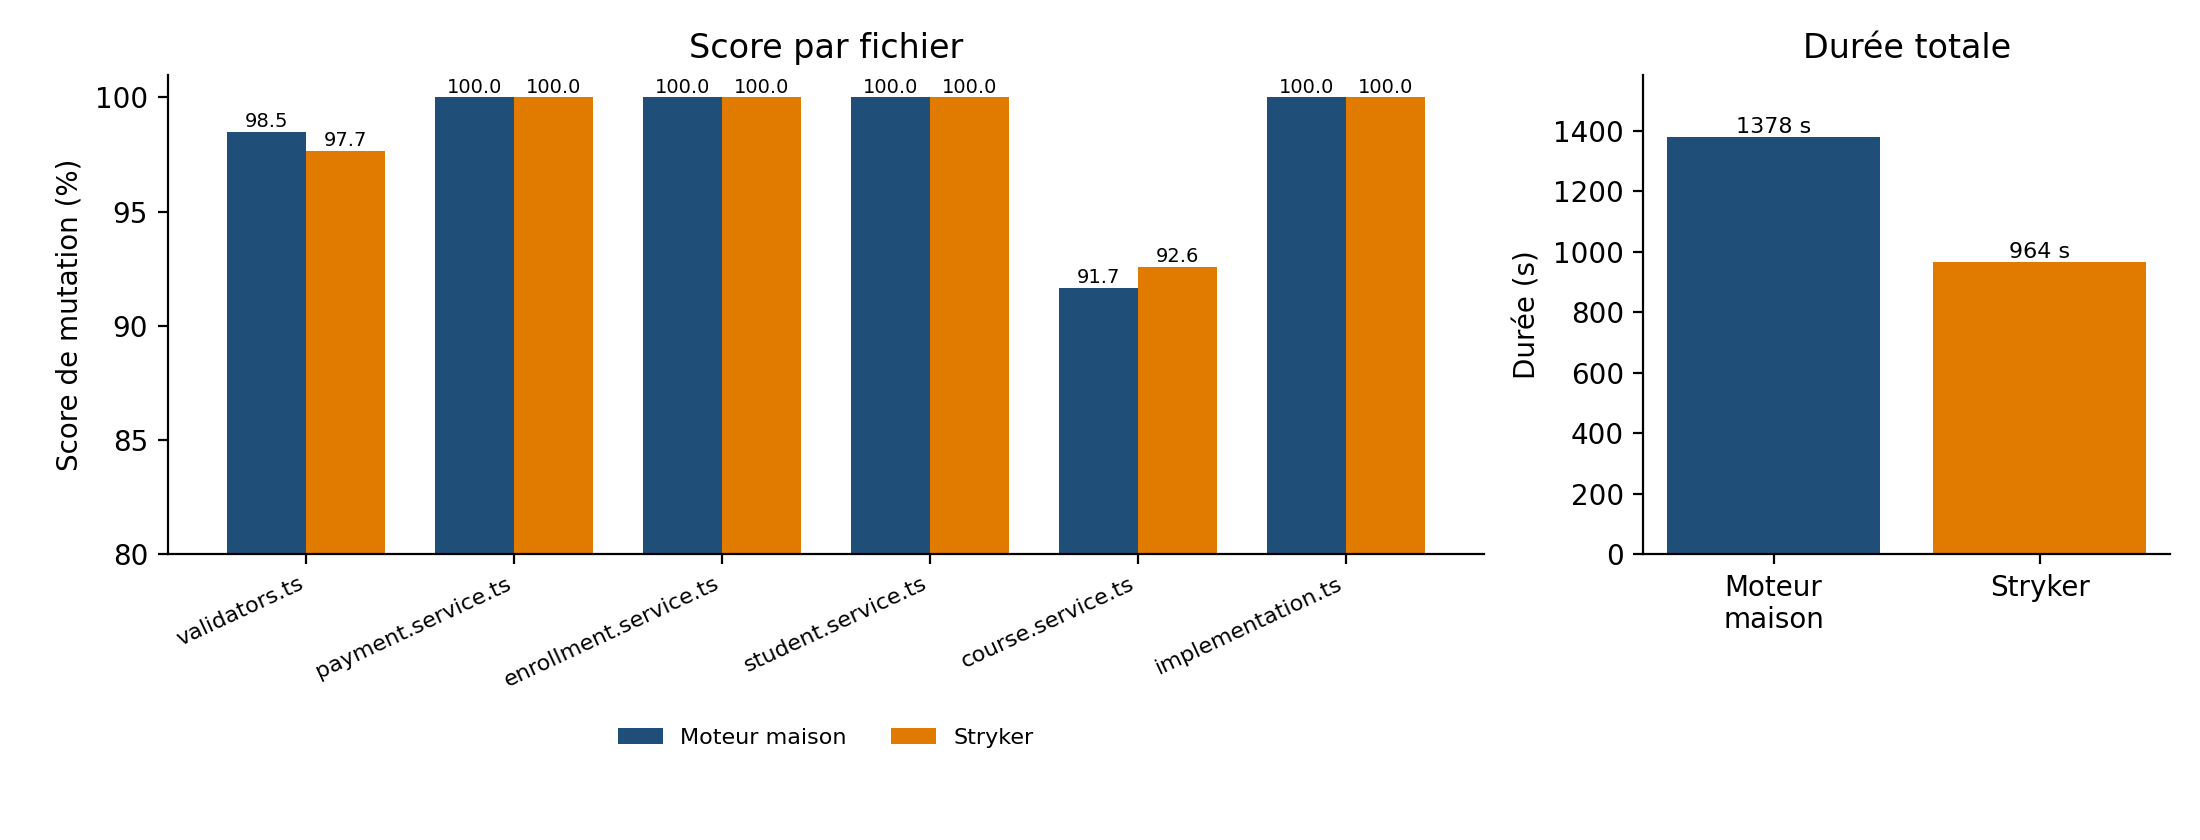
\includegraphics[width=\textwidth]{fig_benchmark_scores.png}}{}
\caption{Score de mutation par fichier et durée totale (l'axe des scores commence à 80\,\%)}
\label{fig:bench-scores}
\end{figure}

\subsection{Conditions réelles de l'exécution de Stryker}
Nous avons exécuté Stryker 10.0.0 (plugin \texttt{@stryker-mutator/vitest-runner} 10.0.0, 7 processus en parallèle) sur les six fichiers. Les tableaux ci-dessus donnent ses résultats. Trois remarques sont nécessaires pour les lire.
\begin{enumerate}
    \item \textbf{Version de Vitest.} Avec Vitest 5.0.5, la version du projet, Stryker ne détecte aucun mutant : sur \texttt{payment.service.ts}, nous avons obtenu 0\,\% (21 survivants sur 21), ce qui contredit les tours 1 à 3. Le plugin est prévu pour Vitest 4.1.x. Nous avons donc lancé Stryker sur une copie du projet avec Vitest 4.1.10 (172 tests réussis). Avec cette version, le même fichier donne 21 mutants tués sur 21. Le moteur maison, lui, a tourné sur le projet d'origine, alors sous Vitest 5.
    \item \textbf{Installation.} Il a fallu installer le paquet avec \texttt{pnpm}, car \texttt{npm i} échoue, et déclarer \texttt{"plugins": ["@stryker-mutator/vitest-runner"]} dans \texttt{stryker.config.json}. Sans cela, Stryker ne trouve pas le plugin. Le moteur maison n'a besoin d'aucune installation.
    \item \textbf{Durées difficiles à comparer.} Stryker travaille sur 7 processus et ne rejoue que les tests qui passent par la ligne mutée (2{,}09 tests par mutant en moyenne). Le moteur maison travaille sur un seul processus et rejoue tous les tests du fichier. L'écart (964\,s contre 1\,378\,s) vient donc autant de cette différence de conception que de la vitesse des outils.
\end{enumerate}

\subsection{Démarche d'analyse des écarts}
Nous traitons chaque écart entre les deux outils comme une limite trouvée au tour précédent :
\begin{enumerate}
    \item un survivant vu par les deux outils confirme une faiblesse connue, ou un équivalent déjà justifié dans \texttt{equivalents.json} ;
    \item un survivant vu par Stryker seulement est soit un \textbf{test manquant} (nous écrivons un test tueur, d'abord sur le code d'origine), soit un \textbf{mutant équivalent} propre à Stryker (nous le justifions par écrit), soit un mutant d'un type que notre moteur ne produit pas (bloc, tableau ou objet vidé) ;
    \item un survivant vu par le moteur maison seulement montre ce que Stryker ne regarde pas, par exemple les nombres.
\end{enumerate}

\subsection{Analyse des écarts}
Les deux outils arrivent presque au même résultat : \textbf{98{,}8\,\%} pour le moteur maison (252 mutants tués sur 255) et \textbf{98{,}6\,\%} pour Stryker (409 sur 415, dont 31 arrêtés par dépassement de délai et comptés comme tués). Stryker produit 63\,\% de mutants en plus, mais n'a que 6 survivants. Dans les deux cas, les fichiers \texttt{payment}, \texttt{enrollment}, \texttt{student} et \texttt{implementation} atteignent 100\,\%. Les tests tueurs du tour 2 ne sont donc pas faits sur mesure pour notre moteur.

\paragraph{Survivant commun (1 ligne).} \texttt{course.service.ts}, ligne 50 (\texttt{if (!course) throw new CourseNotFoundException}). Stryker y voit deux survivants : la condition remplacée par \texttt{false}, et la levée de l'exception supprimée. Nous avions déjà classé ce mutant comme équivalent au tour 3 : si le cours n'existe pas, \texttt{courseRepository.update} lève exactement la même exception. Stryker arrive à la même conclusion.

\paragraph{Survivants du moteur maison seulement (2 lignes).} Il s'agit de \texttt{validators.ts}, ligne 23 (\texttt{+} devient \texttt{*} dans l'expression régulière) et ligne 36 (\texttt{>} devient \texttt{>=}). Ce sont deux de nos trois équivalents justifiés. Stryker ne produit pas la mutation de la ligne 23. À la ligne 36, il génère bien \texttt{digit >= 9}, mais le classe \og délai dépassé \fg{} (\emph{timeout}), donc tué, alors que ce mutant est équivalent. Cela vient sans doute du délai de 10\,s avec 7 processus en parallèle, et non d'une vraie détection. Le score de Stryker est donc un peu trop favorable, et nous n'avons pas vérifié un par un ses 31 mutants en \emph{timeout}.

\paragraph{Survivants de Stryker seulement (4 lignes).}
\begin{itemize}
    \item \texttt{validators.ts}, lignes 84 (\texttt{getCardType}) et 92 (\texttt{maskCardNumber}) : le remplacement de la chaîne vide par \texttt{"Stryker was here!"} dans \texttt{replace(/\textbackslash D/g, '')} survit. Le résultat ne change que si le numéro \textbf{commence} (pour \texttt{getCardType}) ou \textbf{finit} (pour \texttt{maskCardNumber}) par un caractère qui n'est pas un chiffre, par exemple un espace. Aucun test ne couvre ce cas. C'est un \textbf{vrai manque de test}, que notre moteur ne pouvait pas voir car il ne modifie pas ce genre de chaîne vide.
    \item \texttt{validators.ts}, ligne 86 : l'expression \texttt{[3-6]\textbackslash d\{2\}} devient \texttt{[3-6]\textbackslash d}. Les deux versions ne diffèrent que pour un numéro de moins de quatre chiffres (par exemple \texttt{getCardType("235")}), un cas que la validation de longueur écarte avant. Un test direct le tuerait, mais dans le fonctionnement réel le mutant est presque équivalent.
    \item \texttt{validators.ts}, ligne 16 : le corps de \texttt{currentYear()} vidé est classé \og sans couverture \fg{}. Nous n'avons pas cherché la cause ; elle vient probablement de la façon dont la date est fixée dans les tests.
\end{itemize}
Nous n'avons pas corrigé ces quatre points dans ce benchmark.

\paragraph{Bilan.}
\begin{itemize}
    \item Notre moteur est confirmé : son score (98{,}8\,\%) est très proche de celui de Stryker (98{,}6\,\%), et ses trois équivalents sont cohérents avec ce que Stryker observe.
    \item Stryker révèle \textbf{deux vrais manques de test} que nous n'avions pas vus : un numéro de carte avec un caractère qui n'est pas un chiffre au début ou à la fin.
    \item Notre moteur trouve des survivants que Stryker ne signale pas (lignes 23 et 36), mais ce sont des équivalents.
    \item Sur cette suite, Stryker est plus rapide (2{,}32\,s contre 5{,}40\,s par mutant) et fournit un rapport HTML pratique. En revanche, il impose une version précise de Vitest.
\end{itemize}

\subsection{Limites du benchmark}
\begin{itemize}
    \item \textbf{Une seule machine, une seule exécution} : les durées varient avec la charge ; elles donnent un ordre de grandeur, pas une mesure statistique.
    \item \textbf{Mutants non comparables un à un} : les deux outils n'ont pas les mêmes mutateurs, donc des totaux différents ne signifient pas que l'un \og trouve plus \fg{} d'erreurs.
    \item \textbf{Compatibilité des versions} : le plugin Vitest de Stryker 10.0.0 est validé avec Vitest 4.1.x ; avec Vitest 5.0.5, les mutants ne sont jamais activés et le score est nul (voir la sous-section \og Conditions réelles de l'exécution de Stryker \fg{}).
    \item \textbf{Environnement jsdom} : la suite crée un environnement jsdom par fichier de test, ce qui pèse sur le temps de chaque mutant, quel que soit l'outil.
\end{itemize}

\end{document}
